% Adapted from the user-supplied Complete_English_Thesis_Template.tex.
% The original file is preserved, unchanged, under template/.
% Run: python build_proposal.py (or latexmk after generate_results.py).
\documentclass[12pt,a4paper,oneside]{report}
\usepackage[T1]{fontenc}
\usepackage[utf8]{inputenc}
\usepackage[english]{babel}
\usepackage{lmodern}
\usepackage[left=32mm,right=25mm,top=27mm,bottom=27mm]{geometry}
\usepackage{setspace}
\onehalfspacing
\usepackage{microtype}
\usepackage{amsmath,amssymb}
\usepackage{graphicx}
\usepackage{booktabs,tabularx,longtable,array}
\usepackage{enumitem}
\usepackage{xcolor}
\usepackage{fancyhdr}
\usepackage{caption}
\usepackage{listings}
\usepackage[numbers,sort&compress]{natbib}
\usepackage{xurl}
\usepackage{hyperref}
\usepackage[nameinlink,noabbrev]{cleveref}
\usepackage{bookmark}
\usepackage{etoolbox}
\usepackage{placeins}
\usepackage{pdflscape}
% User-supplied academic details. Leave optional fields empty to omit them.
\newcommand{\ThesisTitle}{Physics-Informed Modeling of Fluid Flow and Particle Transport in Curved Channels}
\newcommand{\ShortTitle}{Physics-Informed Particle Transport}
\newcommand{\AuthorName}{Mohammad Reza Sayah}
\newcommand{\UniversityName}{Sharif University of Technology}
\newcommand{\DegreeName}{Master of Science}
\newcommand{\SupervisorName}{Mohammad Ali Bijarchi}
\newcommand{\DepartmentName}{}
\newcommand{\StudentID}{}
\newcommand{\CoSupervisorName}{}
\newcommand{\SubmissionDate}{October 2026}

% Generated numerical evidence.
\newcommand{\FlowVelocityPercent}{1.510}
\newcommand{\FlowPressurePercent}{0.863}
\newcommand{\DragPercent}{0.717}
\newcommand{\PoiseuilleVelocityPercent}{0.217}
\newcommand{\PoiseuillePressurePercent}{0.180}
\newcommand{\ABCVelocityPercent}{2.428}
\newcommand{\ABCPressurePercent}{13.501}
\newcommand{\FluxPercent}{2.266}
\newcommand{\MeshDifferencePercent}{0.173}
\newcommand{\InterpolationPercent}{0.177}
\newcommand{\VelocityMeanPercent}{1.469}
\newcommand{\VelocitySDPercent}{0.057}
\newcommand{\MaxPathWidthPercent}{34.973}
\newcommand{\MinimumTimeCoveragePercent}{73.553}
\newcommand{\MaximumParticleRe}{0.01221}
\newcommand{\BaselineAgreement}{6}
\newcommand{\BaselineCount}{7}
\newcommand{\TotalIntegrations}{119}
\newcommand{\ParticleIntegrations}{105}
\newcommand{\TracerIntegrations}{14}
\newcommand{\FailedIntegrations}{0}
\newcommand{\CompletedStages}{35}
\newcommand{\FailedStages}{0}
\newcommand{\ChannelWidth}{0.30}
\newcommand{\ChannelLength}{2.1991}
\newcommand{\ReynoldsNumber}{1.0}
\newcommand{\InnerRadius}{0.20}
\newcommand{\OuterRadius}{0.50}
\newcommand{\BaselineDiameter}{0.025}
\newcommand{\BaselineDensity}{1000}
\newcommand{\FinestTriangles}{3026}
\newcommand{\EvidenceRevision}{97d71480fc01}
\newcommand{\EvidenceRevisionFull}{97d71480fc012b04a2265368c1e13f54512b694b}

\graphicspath{{../results/final_study/figures/}}

\expandafter\def\csname EvidenceTablesummary\endcsname{
Curved channel & Velocity relative error & 1.510\% \\
Curved channel & Pressure relative error & 0.863\% \\
Drag network & Held-out normalized force error & 0.717\% \\
Poiseuille PINN & Velocity relative error & 0.217\% \\
Poiseuille PINN & Pressure relative error & 0.180\% \\
Poiseuille FEM & Velocity relative error & $8.192\times 10^{-10}$ \\
Finest FEM pair & Velocity difference & 0.173\% \\
Reference interpolation & Velocity difference & 0.177\% \\
Baseline particle outcomes & Matched endpoint classes & 6/7 \\
ABC benchmark & Velocity relative error & 2.428\% \\
ABC benchmark & Pressure relative error & 13.501\% \\
}
\expandafter\def\csname EvidenceTablemesh\endcsname{
30 $\times$ 6 & 290 & 1.141 & $2.448\times 10^{-1}$ \\
60 $\times$ 12 & 1298 & 0.173 & $7.819\times 10^{-2}$ \\
90 $\times$ 18 & 3026 & 0.000 & $4.128\times 10^{-2}$ \\
}
\expandafter\def\csname EvidenceTableseeds\endcsname{
42 & 1.510 & 0.863 \\
43 & 1.429 & 0.886 \\
}
\expandafter\def\csname EvidenceTabletrajectories\endcsname{
-0.650 & 2.668 & 98.86 & Yes \\
-0.433 & 2.299 & 99.33 & Yes \\
-0.217 & 4.298 & 99.27 & Yes \\
0.000 & 7.834 & 98.59 & Yes \\
0.217 & 16.086 & 96.19 & Yes \\
0.433 & 34.973 & 87.39 & Yes \\
0.650 & 3.295 & 73.55 & No \\
}
\expandafter\def\csname EvidenceTableoutcomes\endcsname{
Baseline & PINN + ForceNet & 6 & 1 & 0 \\
Baseline & FEM + Stokes & 7 & 0 & 0 \\
$d_p=0.0105$ & PINN + ForceNet & 7 & 0 & 0 \\
$d_p=0.0105$ & FEM + Stokes & 7 & 0 & 0 \\
$d_p=0.0255$ & PINN + ForceNet & 6 & 1 & 0 \\
$d_p=0.0255$ & FEM + Stokes & 7 & 0 & 0 \\
$d_p=0.045$ & PINN + ForceNet & 0 & 7 & 0 \\
$d_p=0.045$ & FEM + Stokes & 0 & 7 & 0 \\
$\rho_r=200$ & PINN + ForceNet & 7 & 0 & 0 \\
$\rho_r=200$ & FEM + Stokes & 7 & 0 & 0 \\
$\rho_r=1000$ & PINN + ForceNet & 6 & 1 & 0 \\
$\rho_r=1000$ & FEM + Stokes & 7 & 0 & 0 \\
$\rho_r=3000$ & PINN + ForceNet & 0 & 7 & 0 \\
$\rho_r=3000$ & FEM + Stokes & 1 & 6 & 0 \\
}
\expandafter\def\csname EvidenceTablesoftware\endcsname{
numpy & 2.3.5 \\
scipy & 1.17.0 \\
torch & 2.14.1+cpu \\
matplotlib & 3.10.8 \\
scikit-fem & 12.0.2 \\
Pillow & 12.3.0 \\
}
\expandafter\def\csname EvidenceTablequality\endcsname{
Analytical FEM & Met \\
Poiseuille PINN velocity & Met \\
Poiseuille PINN pressure & Met \\
FEM nonlinear solve & Met \\
Reference mesh sensitivity & Met \\
Reference interpolator & Met \\
Channel velocity & Met \\
Channel pressure & Met \\
Velocity boundary & Met \\
Channel mass flux & Met \\
Drag surrogate & Met \\
Trajectory integration & Met \\
Particle endpoint agreement & Not met \\
Particle position error & Not met \\
Trajectory time coverage & Not met \\
ABC velocity & Met \\
ABC pressure & Not met \\
Execution stages & Met \\
}

\newcommand{\TableRows}[1]{\csname EvidenceTable#1\endcsname}
\definecolor{ThesisBlue}{HTML}{173F5F}
\hypersetup{colorlinks=true,linkcolor=ThesisBlue,citecolor=ThesisBlue,urlcolor=ThesisBlue,
  pdftitle={\ThesisTitle},pdfauthor={\AuthorName},
  pdfsubject={Master of Science research proposal with preliminary numerical evidence}}
\setcounter{secnumdepth}{2}
\setcounter{tocdepth}{1}
\setlength{\headheight}{15pt}
\pagestyle{fancy}
\fancyhf{}
\fancyhead[L]{\small\ShortTitle}
\fancyhead[R]{\small Research Proposal}
\fancyfoot[C]{\thepage}
\renewcommand{\headrulewidth}{0.3pt}
\fancypagestyle{plain}{\fancyhf{}\fancyfoot[C]{\thepage}\renewcommand{\headrulewidth}{0pt}}
\setlist[itemize]{topsep=4pt,itemsep=2pt,parsep=0pt}
\setlist[enumerate]{topsep=4pt,itemsep=3pt,parsep=0pt}
\captionsetup{font=small,labelfont=bf}
\renewcommand{\arraystretch}{1.15}
\newcolumntype{Y}{>{\raggedright\arraybackslash}X}
\lstset{basicstyle=\ttfamily\footnotesize,breaklines=true,frame=single,
  columns=fullflexible,keepspaces=true,showstringspaces=false}
\newcommand{\FrontChapter}[1]{\chapter*{#1}\phantomsection
  \addcontentsline{toc}{chapter}{#1}\markboth{#1}{#1}}
\newcommand{\ResultFigure}[5][0.94]{%
  \begin{figure}[!htbp]\centering
  \includegraphics[width=#1\textwidth,height=0.60\textheight,keepaspectratio]{#2.pdf}
  \caption[#3]{#4}\label{#5}\end{figure}}
\newcommand{\WideResultFigure}[4]{%
  \begin{landscape}\begin{figure}[p]\centering
  \includegraphics[width=.98\linewidth,height=.72\textheight,keepaspectratio]{#1.pdf}
  \caption[#2]{#3}\label{#4}\end{figure}\end{landscape}}
\newcommand{\vect}[1]{\boldsymbol{#1}}
\newcommand{\MSE}{\operatorname{MSE}}
\newcommand{\Rey}{\mathrm{Re}}
\newcommand{\St}{\mathrm{St}}
\setlength{\emergencystretch}{1.5em}
\begin{document}
\hypersetup{pageanchor=false}
\begin{titlepage}
\centering
\vspace*{7mm}
{\Large\UniversityName\par}
\ifdefempty{\DepartmentName}{}{\vspace{3mm}{\large\DepartmentName\par}}
\vspace{17mm}
{\Huge\bfseries\color{ThesisBlue}\ThesisTitle\par}
\vspace{12mm}
{\Large Research Proposal\par}
\vspace{4mm}
{\large\DegreeName\par}
\vspace{13mm}
{\Large\AuthorName\par}
\ifdefempty{\StudentID}{}{\vspace{3mm}Student ID: \StudentID\par}
\vspace{9mm}
{\large Supervisor: \SupervisorName\par}
\ifdefempty{\CoSupervisorName}{}{Co-supervisor: \CoSupervisorName\par}
\vfill
{\small Preliminary computational evidence and proposed research plan\par}
\vspace{5mm}
{\normalsize\SubmissionDate\par}
\end{titlepage}
\pagenumbering{roman}
\hypersetup{pageanchor=true}
\FrontChapter{Abstract}
Reliable prediction of particle transport in curved channels requires both
an accurate fluid field and a faithful treatment of particle inertia and
wall contact. This proposal develops a physics-informed neural-network
workflow for steady incompressible flow and dilute spherical-particle
transport, with independent numerical references and explicit accuracy
criteria. A flow network with five hidden layers of 70 neurons predicts
velocity and pressure; a force network with five hidden layers of 90 neurons
approximates the specified Stokes-drag relation. Existing repository results
provide preliminary evidence: the principal curved-channel case has velocity
and pressure errors of \FlowVelocityPercent\% and \FlowPressurePercent\%
relative to an independently assembled finite-element reference. Across two
training seeds, the mean velocity error is \VelocityMeanPercent\%. However,
only \BaselineAgreement\ of \BaselineCount\ baseline particle endpoint
classes agree with the reference, and some trajectory errors exceed the
current screening limits. A separate three-dimensional manufactured
benchmark gives velocity and pressure errors of \ABCVelocityPercent\% and
\ABCPressurePercent\%, respectively. These findings motivate a research
program focused on near-wall accuracy, trajectory-based evaluation,
controlled geometry studies, and pressure recovery. The proposed study will
separate numerical verification from physical validation and will evaluate
generalization only on explicitly held-out cases. The expected contribution
is a reproducible, bounded assessment of when physics-informed flow
approximations support reliable particle-transport predictions.

\vspace{4mm}
\noindent\textbf{Keywords:} physics-informed neural networks; particle
transport; curved channels; Stokes drag; numerical verification.

\FrontChapter{Document and Evidence Record}
This is a research proposal supported by existing preliminary computations.
Completed numerical results appear in \cref{ch:preliminary}; the experiments
and improvements in \cref{ch:plan} are proposed work. No experimental
measurements or completed three-dimensional channel study are claimed.

The document adapts the layout, typography, margins, front matter, and
chapter-based structure of the supplied English thesis template. The original
template is retained with the source. Thesis approval, originality-signature,
and completion pages are omitted because they do not describe this proposal.
The author and supervisor details were supplied for the title page.

Numerical tables and highlighted values are generated from
\path{results/final_study/metrics.json} and associated CSV/JSON files.
All 21 research figures are read from the repository's existing PDF exports.
The evidence data revision is \texttt{\EvidenceRevision}. A machine-readable
input hash record accompanies the source. The document build does not
retrain models or alter numerical results.

\noindent\textbf{Repository:}\par
\url{https://github.com/mohrezsayeh90-ai/basic_particle_problem}

\clearpage\phantomsection\addcontentsline{toc}{chapter}{Contents}\tableofcontents
\clearpage\phantomsection\addcontentsline{toc}{chapter}{List of Figures}\listoffigures
\clearpage\phantomsection\addcontentsline{toc}{chapter}{List of Tables}\listoftables
\FrontChapter{Abbreviations and Nomenclature}
\begin{tabularx}{\textwidth}{@{}lY@{}}
\toprule Abbreviation & Meaning\\\midrule
ABC & Arnold--Beltrami--Childress manufactured flow\\
CFD & Computational fluid dynamics\\
FEM & Finite-element method\\
MLP & Multilayer perceptron\\
ODE / PDE & Ordinary / partial differential equation\\
PINN & Physics-informed neural network\\
RMS & Root-mean-square\\
\bottomrule
\end{tabularx}
\vspace{7mm}
\begin{tabularx}{\textwidth}{@{}lY@{}}
\toprule Symbol & Meaning\\\midrule
$L_0,U_0,T_0$ & Reference length, speed, and time; $T_0=L_0/U_0$\\
$\vect{u},p$ & Dimensionless fluid velocity and pressure\\
$\vect{x}_p,\vect{v}_p$ & Dimensionless particle position and velocity\\
$R_{\rm in},R_{\rm out}$ & Nominal inner and outer radii of the arc channel\\
$h,W,L$ & Channel half-width, width $W=2h$, and centerline length\\
$s,\eta$ & Centerline coordinate and normalized transverse coordinate\\
$d_p,\rho_r$ & Dimensionless particle diameter and density ratio $\rho_p/\rho_f$\\
$\Rey,\Rey_p,\St$ & Reference Reynolds number, particle Reynolds number, Stokes number\\
$\vect{F}^{*}$ & Drag force scaled by displaced-fluid mass times $U_0^2/L_0$\\
$\theta,\phi$ & Parameters of the flow and force networks\\
$Q,Q_0$ & Section flux and prescribed reference flux\\
\bottomrule
\end{tabularx}
\clearpage\pagenumbering{arabic}
\chapter{Introduction}
\label{ch:introduction}
\section{Background and Problem}
Curved channels couple fluid turning with particle inertia. A fluid marker
follows the local velocity, whereas a finite-inertia particle can lag behind
a change in flow direction and approach a wall. Predicting the resulting
trajectory is relevant to transport, separation, and deposition studies.
The mathematical difficulty is broader than approximating a smooth velocity
field: small, spatially localized errors can change a discrete outcome such
as whether a particle exits or sticks.

Physics-informed neural networks incorporate governing-equation and boundary
residuals into a learning objective \cite{raissi2019,karniadakis2021}. They
offer a differentiable approximation that can be evaluated during trajectory
integration. Their optimization, scaling, and accuracy nevertheless require
verification; a small loss or an attractive plot is insufficient evidence
of a reliable solution \cite{wang2021,wang2022}. Classical CFD remains a
necessary independent comparator in the present study.

The current project already includes a two-network implementation, analytical
tests, an independent FEM reference, and particle tracking. Its preliminary
results reveal a useful research problem: the principal flow approximation
has a relatively small mean error, yet some particle paths and endpoint
classes differ from the reference. This proposal therefore studies the
connection between field accuracy and transport accuracy, rather than
assuming one implies the other.

\section{Aim and Objectives}
The aim is to develop and assess a reproducible physics-informed workflow
for predicting dilute-particle transport in smooth curved channels within
an explicitly defined physical and geometric scope.
\begin{enumerate}[label=O\arabic*.]
\item Quantify flow and pressure accuracy against analytical and independently
assembled numerical references, including mesh and interpolation sensitivity.
\item Determine how local field errors, inertia, particle size, and wall
clearance affect trajectory errors and endpoint classification.
\item Evaluate targeted changes to training and sampling using separate
development and final evaluation cases.
\item Establish the supported scope of geometry variation and a distinct
three-dimensional verification pathway, without inferring universal
generalization from the network input dimensions.
\end{enumerate}

\section{Research Questions}
\begin{enumerate}[label=RQ\arabic*.]
\item Under which training and reference-resolution conditions does the
flow PINN satisfy both field-error and mass-conservation criteria?
\item How does flow-approximation error propagate into particle position,
residence time, and sticking or exit decisions?
\item Does a learned force surrogate materially change trajectories compared
with exact Stokes drag evaluated on the same learned flow?
\item Which conclusions persist across separately trained channel shapes and
Reynolds numbers, and what further evidence is needed for a 3D channel model?
\end{enumerate}
The working expectation is that near-wall and turning-region accuracy will
be more informative for deposition than a global sampled velocity norm.
This is a testable hypothesis for the proposed study, not a mechanism
already established by the preliminary figures.

\section{Scope and Intended Contribution}
The initial physical model is steady, incompressible, Newtonian flow with
one-way coupling to dilute, heavy, spherical particles. Stokes drag and
irreversible wall sticking are retained. The supported channel family has
a smooth, nonintersecting planar centerline and constant width. Sharp
corners, junctions, variable-width networks, particle--particle forces,
and feedback on the fluid are outside the present implementation.

The intended contribution is a reproducible evaluation linking field errors
to transport errors. Its scope excludes a universal drag law and arbitrary
3D geometry. The remaining chapters develop the foundations, methods,
evaluation, preliminary evidence and proposed work.

\chapter{Literature and Research Rationale}
\label{ch:literature}
\section{Physics-Informed Flow Approximation}
Raissi et al.\ formulate PINNs by penalizing differential-equation residuals
alongside observed or prescribed information \cite{raissi2019}. The broader
physics-informed learning framework includes several ways to combine
physical constraints and learned approximations \cite{karniadakis2021}.
For this project, the relevant distinction is between a network trained on
PDE and boundary information and a regression model trained directly on
interior CFD labels. The current flow model uses the former design, and its
FEM interior samples are reserved for numerical comparison.

Optimization behavior limits this approach. Gradient imbalance among loss
terms and unequal learning rates of solution components have been studied
in PINNs \cite{wang2021,wang2022}. These results motivate scaling the
momentum and continuity residuals, retaining fixed monitoring samples, and
reporting boundary and flux errors separately. They do not establish that
any particular optimizer or architecture will be accurate in the proposed
curved-channel problem.

\section{Independent Flow and Particle References}
Mixed finite elements provide a classical route to incompressible flow.
The Taylor--Hood construction uses a higher-order velocity space than
pressure space \cite{taylor1973}; the present independent reference uses
P2 velocity and P1 pressure with scikit-fem \cite{gustafsson2020}.
Independence here means that this solver is assembled without PINN
predictions. Its own nonlinear, mesh, and continuity checks remain necessary.
It is a project-specific CFD reference, not a claim that commercial CFD or
an experimental benchmark was used.

The full small-sphere equation of motion includes terms beyond instantaneous
Stokes drag \cite{maxey1983}. The present model deliberately uses a
heavy-particle simplification. This is appropriate only within a qualified
regime and cannot represent every particle--fluid interaction. In particular,
geometric wall contact does not supply the hydrodynamic wall corrections
that may become important at small clearances.

\section{Verification, Validation, and the Specific Gap}
Numerical verification addresses consistency with the stated equations;
physical validation concerns agreement with suitable external physical
evidence \cite{roache1998}. Analytical Poiseuille flow and a manufactured
three-dimensional solution are strong implementation checks. Agreement with
a refined FEM solution tests numerical consistency for the same model.
Neither substitutes for experiment when making device-level predictions.

\begin{table}[!htbp]
\centering\small
\caption{Roles of the main methodological foundations.}
\label{tab:literature}
\begin{tabularx}{\textwidth}{@{}p{.23\textwidth}YY@{}}
\toprule Foundation & Role in this proposal & Limit of inference\\\midrule
PINNs \cite{raissi2019,karniadakis2021} & Differentiable flow approximation constrained by physics & Training loss does not certify trajectory accuracy.\\
Training analysis \cite{wang2021,wang2022} & Motivation for loss scaling and separate diagnostics & Remedies must be evaluated on this channel family.\\
Taylor--Hood FEM \cite{taylor1973} & Independent velocity/pressure reference & Discretization and geometry errors remain.\\
Small-sphere dynamics \cite{maxey1983} & Basis for the drag-only heavy-particle model & Other force terms and confinement are omitted.\\
Numerical verification \cite{roache1998} & Reference hierarchy and error reporting & Numerical agreement is not experimental validation.\\
\bottomrule
\end{tabularx}
\end{table}

The proposed gap is local to the current workflow: its global field metrics
and particle-outcome metrics do not yet support the same level of confidence.
The study will investigate that discrepancy and determine a defensible
operating envelope. This is a focused narrative rationale based on the cited
foundational work and repository evidence; it is not presented as an
exhaustive or systematic survey of all particle-transport PINNs.

\chapter{Physical and Mathematical Framework}
\label{ch:theory}
\section{Geometry and Nondimensionalization}
The default S-channel joins two semicircular segments with a continuous
tangent and piecewise curvature. Its nominal radii are
$R_{\rm in}=\InnerRadius$ and $R_{\rm out}=\OuterRadius$; the centerline
radius is their average. The width is $W=R_{\rm out}-R_{\rm in}=\ChannelWidth$
and the centerline length is approximately $L=\ChannelLength$.
A general supported channel is represented by
\begin{equation}
 \vect{x}(s,\eta)=\vect{c}(s)+h\eta\vect{n}(s),\qquad
 0\le s\le L,\quad -1\le\eta\le1,\quad h=W/2,
 \label{eq:geometry}
\end{equation}
where $\vect{c}$ is a planar centerline and $\vect{n}$ its unit normal.
Curvature and overlap checks exclude invalid offset tubes. A custom CSV
changes the centerline, not the physical topology supported by the solver.

Dimensional variables are scaled using $L_0$, $U_0$ and $\mu U_0/L_0$ for
length, speed and pressure. Time is scaled by $T_0=L_0/U_0$. Throughout the
following equations, variables without a dimensional subscript are
dimensionless. The reference Reynolds number is
$\Rey=\rho_f U_0 L_0/\mu$; $L_0$ is not implicitly a hydraulic diameter.
The current principal case uses $\Rey=\ReynoldsNumber$.

\ResultFigure{01_geometry}{Channel and sampling}{Default channel and sampled
interior and boundary points from the repository. Coordinates are
nondimensional; the displayed point set illustrates the sampling procedure.}{fig:geometry}

\section{Fluid Equations and Boundary Conditions}
For a steady incompressible Newtonian fluid,
\begin{align}
 \nabla\cdot\vect{u}&=0,\label{eq:continuity}\\
 \Rey(\vect{u}\cdot\nabla)\vect{u}&=-\nabla p+\nabla^2\vect{u}.
 \label{eq:momentum}
\end{align}
The walls satisfy no slip. Both end sections have the prescribed tangential
velocity $\vect{u}=(1-\eta^2)\vect{t}$ with unit center speed. Pressure has
one gauge condition. In particular, the outlet is a prescribed-velocity
boundary, rather than an assumed zero-pressure outlet. The FEM and PINN use
these same physical boundary conditions, with their pressure constants
aligned during comparison. The prescribed section flux is $Q_0=4h/3$.

\section{Particle and Fluid-Marker Dynamics}
Let $d_p$ be particle diameter and $\rho_r=\rho_p/\rho_f$ the density ratio.
The adopted drag-only heavy-particle equations are
\begin{align}
 \frac{d\vect{x}_p}{dt}&=\vect{v}_p,\label{eq:particle-position}\\
 \frac{d\vect{v}_p}{dt}&=\frac{18}{\rho_r\Rey d_p^2}
 [\vect{u}(\vect{x}_p)-\vect{v}_p]
 =\frac{\vect{u}(\vect{x}_p)-\vect{v}_p}{\St},
 \qquad \St=\frac{\rho_r\Rey d_p^2}{18}.
 \label{eq:particle-velocity}
\end{align}
The particle Reynolds number is
$\Rey_p=\Rey d_p\lVert\vect{u}-\vect{v}_p\rVert$.
Stokes drag requires $\Rey_p\ll1$ and a particle small relative to flow
length scales. The force formulation is a simplification of small-sphere
dynamics, not the full Maxey--Riley equation \cite{maxey1983}.

A fluid marker follows $d\vect{x}/dt=\vect{u}(\vect{x})$. A finite-size
particle sticks when its center reaches a distance $d_p/2$ from the wall;
its velocity is then set to zero. This contact rule is irreversible and
does not represent rebound or adhesion-force calibration. Initial particle
velocity equals the local fluid velocity unless the user supplies a
different admissible value.

\section{Force-Network Interpretation}
The normalized drag force $\vect{F}^{*}$ is scaled by displaced-fluid mass
times $U_0^2/L_0$. With input
$z=(u,v,p,d_p,x_p,y_p,u_p,v_p)$ and normalized input map $N$, the implemented
surrogate is
\begin{equation}
 \widehat{\vect{F}}^{*}(z)=\frac{18}{\Rey d_p^2}
 \{g_\phi(Nz)-g_\phi(Nz_0)\},
 \label{eq:force-network}
\end{equation}
where $z_0$ replaces the particle velocity by the fluid velocity. Subtraction
enforces zero force at zero slip. The network is trained against the
algebraic Stokes residual, so it approximates an already specified law.
Pressure and particle position are input slots; they do not establish
additional force mechanisms. Exact Stokes drag remains the reference.

\section{Physical Limits}
The model omits gravity, lift, Brownian motion, added mass, history effects,
fluid feedback, particle collisions, and near-wall lubrication corrections.
The largest tested diameter is 15\% of the channel width, so that case is a
sensitivity study rather than proof of the unbounded point-particle model's
physical accuracy. The computed maximum $\Rey_p$ is
\MaximumParticleRe; this supports a low-slip-inertia regime but does not
remove confinement or dilute-loading assumptions.

\chapter{Computational Methodology}
\label{ch:methods}
\section{Architecture and Training}
The flow network maps $(x,y,R_{\rm in},R_{\rm out},\Rey)$ to $(u,v,p)$
through five hidden layers of 70 tanh units. The force network maps the eight
inputs in \cref{eq:force-network} to two force components through five hidden
layers of 90 tanh units. Spatial coordinates are affinely normalized, and
the pressure output uses a scale $p_s=2L/h^2$.

\begin{figure}[p]\centering
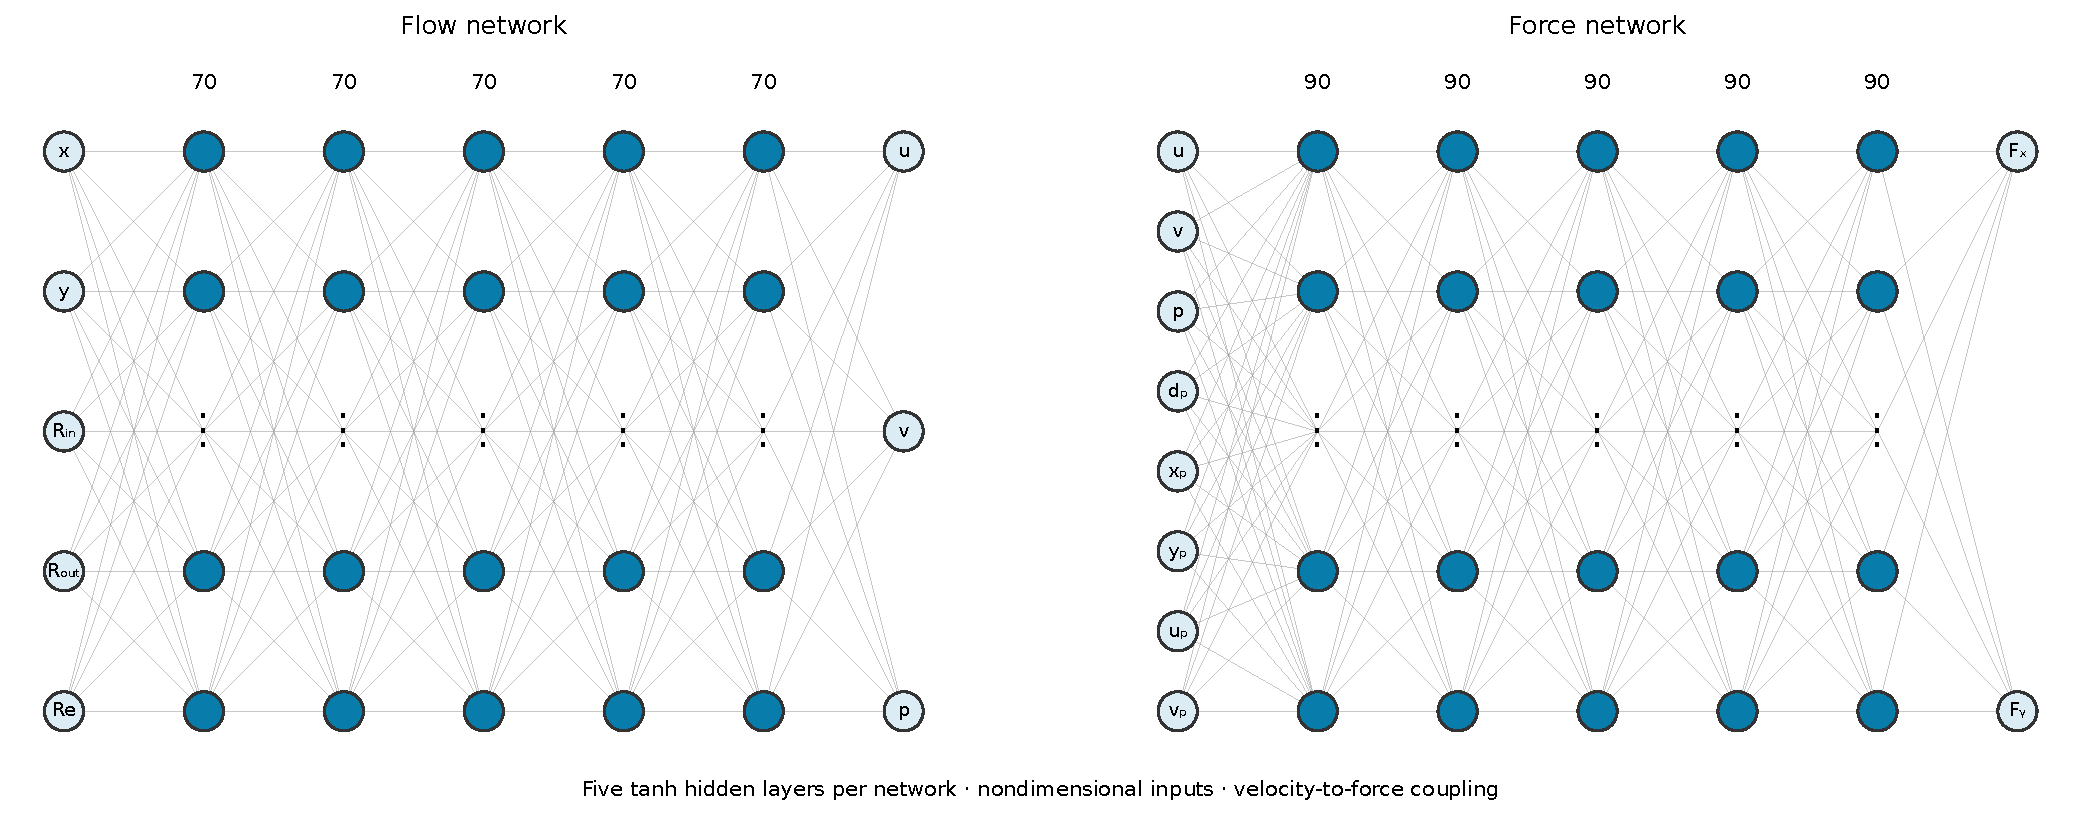
\includegraphics[width=.9\textwidth,trim=0 22 499.535 0,clip]{02_architecture.pdf}\par
\vspace{2mm}
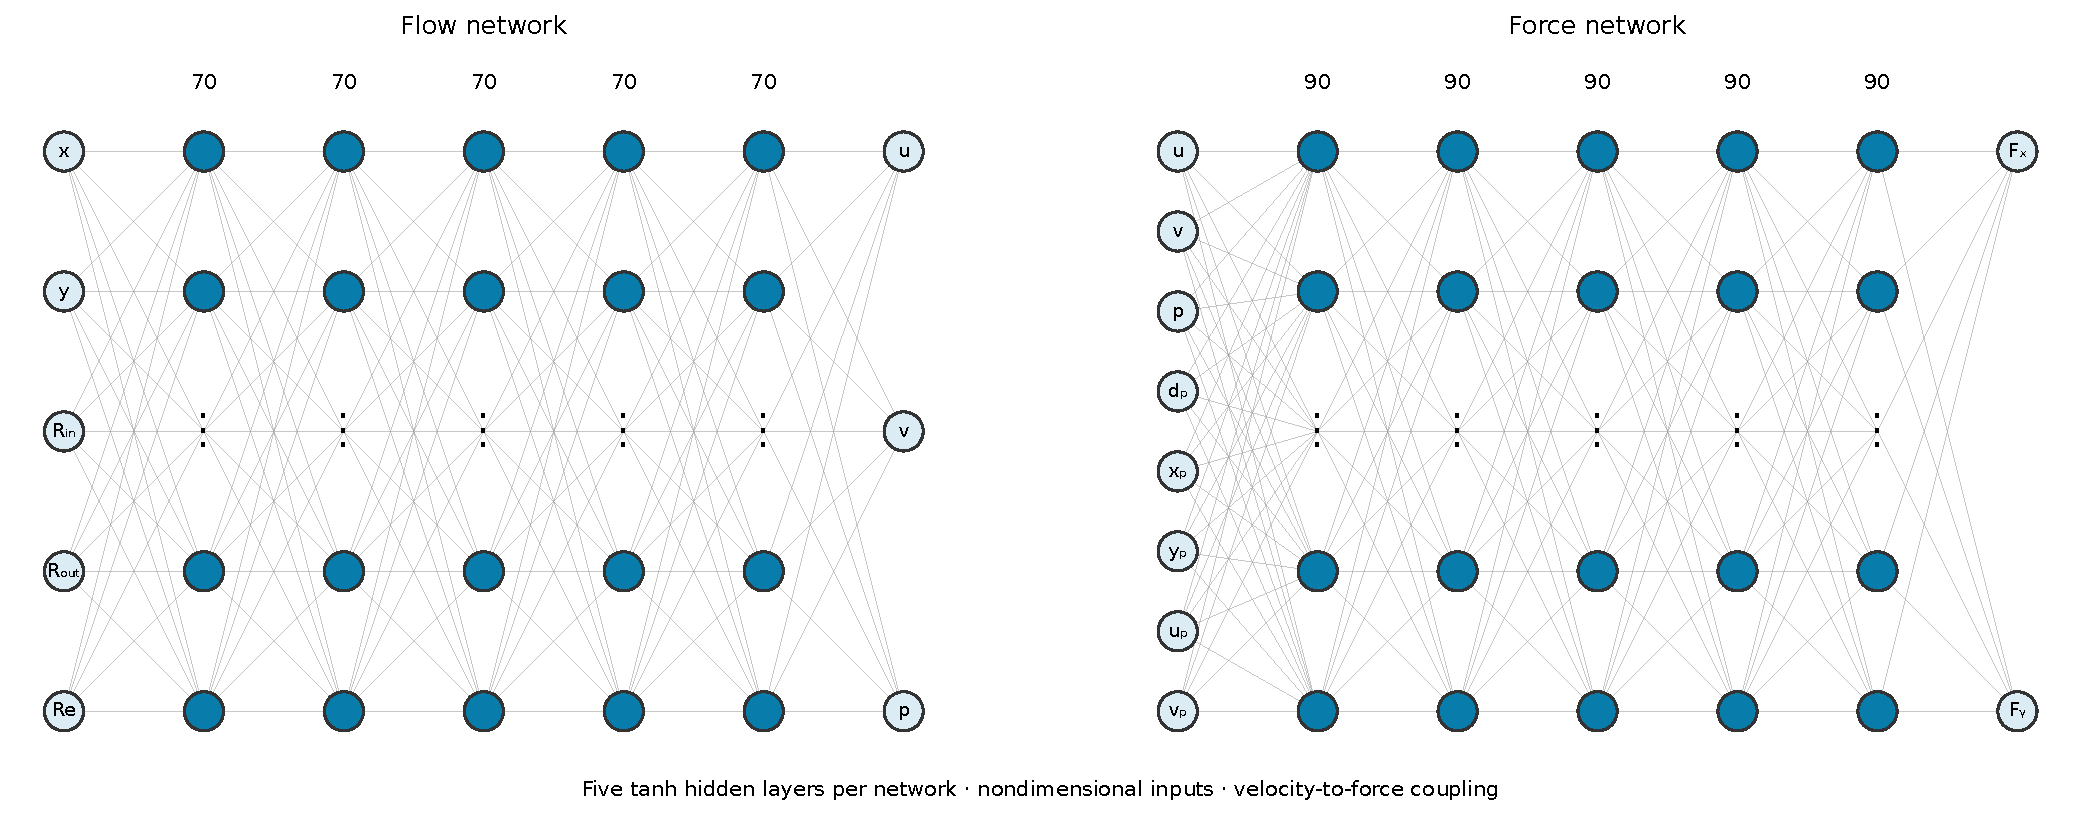
\includegraphics[width=.9\textwidth,trim=499.535 22 0 0,clip]{02_architecture.pdf}
\caption[Network architecture]{Flow network (top) and force network (bottom),
shown as enlarged crops of the existing architecture PDF. Five hidden
layers contain 70 and 90 units, respectively. Dots abbreviate neurons;
labels give actual layer widths.}\label{fig:architecture}
\end{figure}

For continuity residual $r_c$ and the two momentum residuals $\vect{r}_m$,
the implemented flow objective is
\begin{align}
 \mathcal L_{\rm flow}={}&\MSE(h r_c)+\MSE(h^2\vect{r}_m)
 +20\MSE(\widehat{\vect{u}}-\vect{u}_{\rm BC})\nonumber\\
 &+(\widehat p_g/p_s)^2
 +5\MSE(Q/Q_0-1).
 \label{eq:flow-loss}
\end{align}
Here the gauge pressure target is zero, and flux is sampled on seven sections
using 25 transverse points per section. This integral mass constraint helps
exclude a low-throughput interior field that would be inconsistent with
the prescribed inlet flux. The force loss is the mean-square residual
between normalized predicted drag and fluid--particle slip.

Interior samples are resampled during Adam training. Fixed PDE-monitor
samples support checkpoint selection, followed by L-BFGS refinement on
fixed collocation samples. Reference FEM interior labels do not enter the
flow-training objective. Each geometry/Reynolds-number case is trained
separately; fixed parameter input slots are not evidence of a parametric
solution across untrained geometries.

\begin{table}[!htbp]
\centering\small
\caption{Recorded settings of the preliminary training run.}
\label{tab:training}
\begin{tabularx}{\textwidth}{@{}lY@{}}
\toprule Item & Recorded setting\\\midrule
Principal flow seeds & 42 and 43; first seed used for the principal comparison\\
Initial flow phase & 1,000 Adam epochs, 512 interior samples per epoch, 250 L-BFGS iteration budget\\
Refinement phase & 1,800 Adam epochs, 1,024 samples per epoch, 700 L-BFGS iteration budget\\
Adam learning rate & $10^{-3}$ with cosine scheduling to $5\times10^{-5}$ per flow phase\\
Force training & 1,000 Adam epochs; batches of 512; learning rate $8\times10^{-4}$\\
Force selection and testing & 1,024 selection samples; separately sampled held-out tests\\
Flow evaluation & 1,600 fixed interior points for direct FEM comparison\\
3D manufactured benchmark & 800 Adam epochs and 400 L-BFGS iteration budget; a separate model\\
\bottomrule
\end{tabularx}
\end{table}
These settings describe the original training recorded in the checkpoint
metadata. The archived final study reloaded those weights to reproduce
evaluation and figures; its default command-line preset fields should not
be mistaken for a second training run.

\section{Independent FEM Reference}
The reference solves \cref{eq:continuity,eq:momentum} on a triangular mesh
constructed from the same centerline and width. Vector P2 velocity and P1
pressure spaces form the Taylor--Hood discretization
\cite{taylor1973,gustafsson2020}. Picard iteration treats the nonlinear
advection term, and each mixed linear system is solved with a sparse direct
solver. The finest recorded mesh has \FinestTriangles\ triangles. Identical
velocity conditions are imposed at the walls and both end sections; the
arbitrary pressure constant is fixed separately.

The curved wall is polygonal in the reference mesh, so mesh refinement
changes both discretization and geometric approximation. Three resolutions
are retained rather than treating a single successful solve as exact.
For repeated trajectory evaluations, a fast interpolator operates in the
channel's longitudinal/transverse coordinates. This prevents interpolation
across the hole inside a bend. Its error is measured against direct FEM
evaluation before trajectory comparisons are interpreted.

\section{Trajectory Integration and Cases}
ODE integration uses RK45 when the relaxation time is sufficiently long
relative to the geometric step limit, and Radau for shorter, stiffer
relaxation scales. The current tolerances are $2\times10^{-6}$ relative and
$2\times10^{-8}$ absolute. Event functions detect wall contact, outlet
crossing and inlet backflow; time and evaluation budgets keep each run
bounded. A failed path remains marked as failed. A finite output is never
silently replaced by the reference trajectory.

The principal particle has $d_p=\BaselineDiameter$ and
$\rho_r=\BaselineDensity$. Seven inlet positions span $\eta=-0.65$ to
$0.65$. Diameter cases use $d_p=0.0105,0.0255,0.045$, and density cases use
$\rho_r=200,1000,3000$. The baseline and the $\rho_r=1000$ control are
deliberately repeated in the output records and are not independent
physical replications.

Three comparisons isolate different error sources:
\begin{enumerate}
\item PINN flow with ForceNet versus FEM flow with exact Stokes drag measures
the complete surrogate transport discrepancy.
\item PINN flow with ForceNet versus the same PINN flow with exact Stokes
drag isolates the force-surrogate contribution.
\item Fluid markers in PINN and FEM fields examine flow-path differences
without particle inertia.
\end{enumerate}
The archive contains \TotalIntegrations\ integrations:
\ParticleIntegrations\ particle trajectories and \TracerIntegrations\
fluid-marker trajectories. They share models and inputs, and are not treated
as independent experimental observations.

\section{Data Provenance and Independence}
All current flow, force, and trajectory data are computational. The principal
evaluation seed is fixed rather than selected by the smallest FEM error.
The two-seed statistics describe observed training variability, with no claim
of a confidence interval or population-level inference. The current study
is developmental: seeing its failures informs the proposed research plan.
A new frozen evaluation set will therefore be used before making final
claims about improvements, as specified in \cref{ch:plan}.

\chapter{Verification and Evaluation Design}
\label{ch:verification}
\section{Reference Hierarchy}
The evaluation proceeds from exact checks to independently discretized
comparisons. This hierarchy separates equation implementation, numerical
approximation, and physical applicability \cite{roache1998}.

For plane Poiseuille flow in a straight channel of half-width $h$,
\begin{equation}
 u=1-(y/h)^2,\qquad v=0,\qquad p=-2x/h^2+C.
 \label{eq:poiseuille}
\end{equation}
This profile checks both FEM and a separately trained straight-channel PINN.
Velocity profiles are compared on a transverse section; relative pressure
errors use points spanning the channel length, because exact pressure has
no transverse variation on a single section.

In a uniform flow, the Stokes relaxation solution provides an independent
particle-ODE check,
\begin{equation}
 \vect v_p(t)=\vect u+
 [\vect v_p(0)-\vect u]\exp(-t/\St).
 \label{eq:relaxation}
\end{equation}
Algebraic drag tests quantify whether ForceNet reproduces its specified law;
they do not validate that law against real particles near a wall.

\section{Field and Trajectory Metrics}
The reported relative field error is a discrete sample norm,
\begin{equation}
 E_u=\frac{\sqrt{\sum_i\lVert\widehat{\vect u}_i-\vect u_i^{\rm ref}\rVert^2}}
 {\sqrt{\sum_i\lVert\vect u_i^{\rm ref}\rVert^2}}.
 \label{eq:relative-error}
\end{equation}
Pressure uses the same construction after each pressure sample set is
mean-centered to remove gauge differences. Interior sampling is in channel
coordinates; the resulting norm is not an exact area-weighted integral.
Maximum velocity error, boundary RMS error, PDE residuals and section flux
provide complementary information. FEM's integrated divergence norm and
PINN's sampled continuity RMS have different definitions and should not be
compared as if they were identical measures.

For a pair of paths, the position RMS is calculated at 150 common-time
samples up to $T_c=\min(T_{\rm PINN},T_{\rm ref})$. Its ratio to width $W$
is reported alongside $T_c/\max(T_{\rm PINN},T_{\rm ref})$ and endpoint-class
agreement. Restricting the time interval can hide disagreement after one
path ends; the coverage and class measures prevent that truncation from
being interpreted as full-path agreement.

\begin{table}[!htbp]
\centering\small
\caption{Numerical screening criteria used to organize the proposal.}
\label{tab:criteria}
\begin{tabularx}{\textwidth}{@{}p{.43\textwidth}Y@{}}
\toprule Quantity & Screening requirement\\\midrule
Channel velocity and pressure & Relative sampled error below 5\% each\\
Straight-channel PINN & Velocity and pressure error below 5\% each\\
Boundary velocity & Dimensionless RMS below 0.02\\
Section mass flux & Maximum relative deviation below 5\%\\
Reference mesh difference & Penultimate-to-finest velocity difference below 2\%\\
Reference trajectory interpolator & Velocity discrepancy below 2\%\\
Force surrogate & Held-out normalized relative error below 5\%\\
Baseline trajectory position & RMS below 5\% of width for every compared seed\\
Baseline endpoint classes & Agreement for every compared seed\\
Common trajectory time & More than 95\% for every compared seed\\
Separate ABC benchmark & Velocity and pressure errors below 5\% each\\
\bottomrule
\end{tabularx}
\end{table}
These are numerical screening choices, not universal engineering tolerances.
The current records are a developmental baseline; this proposal does not
claim that the listed thresholds were preregistered before all preliminary
inspection. Final acceptance criteria and held-out cases will be frozen
before the proposed comparison experiments begin.

\section{Separate Three-Dimensional Benchmark}
The exact ABC field, with unit amplitudes, is
\begin{align}
 \vect u&=(\sin z+\cos y,\ \sin x+\cos z,\ \sin y+\cos x),\nonumber\\
 p&=-\Rey\lVert\vect u\rVert^2/2,\qquad \vect f=\vect u,
 \label{eq:abc}
\end{align}
on $[0,2\pi]^3$. It satisfies the forced steady momentum equation
$\Rey(\vect u\cdot\nabla)\vect u=-\nabla p+\nabla^2\vect u+\vect f$.
Indeed, $\nabla\cdot\vect u=0$, $\nabla\times\vect u=\vect u$, and
$\nabla^2\vect u=-\vect u$. The convective term is the gradient of
$\lVert\vect u\rVert^2/2$, which is canceled by the pressure gradient.

A separate 3D network predicts all three velocity components and pressure;
known velocity is prescribed on the cube faces, and one pressure value fixes
the gauge. The exact interior field is reserved for evaluation. Particle-free
tracer paths use the periodically extended exact or learned velocity. This
tests genuine 3D derivatives and trajectories, but not a finite-depth curved
channel with sidewalls. The extruded planar channel illustration has an
entirely different role and is identified as visualization only.

\section{Uncertainty and Physical Validation}
The current error budget includes reference mesh and geometry error,
interpolator error, PINN approximation, optimizer variability and ODE error.
Two seeds and a three-mesh comparison do not constitute a formal uncertainty
analysis or a grid-convergence index. Temporal and event-location refinement
are required in the proposed work. At present, no measurement dataset has
been supplied; physical validation and uncertain particle properties remain
open requirements before a device-level claim is justified.

\chapter{Preliminary Results and Interpretation}
\label{ch:preliminary}
\section{Completed Evidence}
The following observations are completed repository results, not outcomes
promised for the proposed study. The archived evaluation completed
\CompletedStages\ stages with \FailedStages\ stage failures and
\FailedIntegrations\ failed integrations. Numerical execution success is
separate from satisfying the accuracy criteria in \cref{tab:criteria}.
\Cref{tab:summary} summarizes the main measurements.

\begin{table}[!htbp]
\centering\small
\caption{Automatically extracted preliminary numerical evidence.}
\label{tab:summary}
\begin{tabularx}{\textwidth}{@{}p{.29\textwidth}Yr@{}}
\toprule Comparison & Metric & Value\\\midrule
\TableRows{summary}
\bottomrule
\end{tabularx}
\end{table}

\section{Analytical and Reference Checks}
\Cref{fig:poiseuille} compares analytical, FEM, and PINN straight-channel
velocity profiles. The PINN velocity error is
\PoiseuilleVelocityPercent\%, while its longitudinally sampled pressure
error is \PoiseuillePressurePercent\%. The FEM velocity error is near
floating-point/iteration accuracy for this polynomial solution. This
verifies the controlled case, not the accuracy of every curved geometry.

\ResultFigure{16_poiseuille_validation}{Poiseuille verification}{Analytical
plane Poiseuille profile with independent FEM and separately trained PINN
profiles. The second panel shows absolute velocity error. Relative pressure
errors are evaluated on longitudinally distributed points, not this section.}{fig:poiseuille}

\begin{table}[!htbp]
\centering\small
\caption{Three reference meshes and their measured sensitivity.}
\label{tab:mesh}
\begin{tabularx}{\textwidth}{@{}lrrY@{}}
\toprule Grid & Triangles & Velocity difference (\%) & $\lVert\nabla\cdot\vect u\rVert_{L^2}$\\\midrule
\TableRows{mesh}
\bottomrule
\end{tabularx}
\end{table}
The penultimate-to-finest velocity difference is
\MeshDifferencePercent\%, and the trajectory interpolator differs from
direct FEM velocity evaluation by \InterpolationPercent\%.
The zero difference in the finest row is a self-comparison; it is not an
estimate of zero discretization error. The declining divergence norm in
\cref{tab:mesh} and the sensitivity plot in \cref{fig:mesh} support reference
refinement, while leaving systematic modeling error unmeasured.

\ResultFigure{08_mesh_sensitivity}{Reference mesh sensitivity}{Velocity
differences to the finest available mesh and the integrated FEM divergence
norm. The plotted floor for the finest self-comparison is a display choice,
not a formal uncertainty estimate.}{fig:mesh}

\section{Curved-Channel Flow}
The principal seed gives sampled velocity and pressure errors of
\FlowVelocityPercent\% and \FlowPressurePercent\%, respectively.
\Cref{fig:fields} compares the spatial fields and errors;
\cref{fig:parity} shows pointwise held-out agreement. Plotting-grid reference
values use the measured fast interpolation; numerical validation metrics
use direct FEM evaluation. Maximum section-flux deviation is
\FluxPercent\%, which is below the present 5\% screen but remains a
nonzero transport inconsistency.

\WideResultFigure{04_flow_fields}{Channel fields and errors}{PINN and FEM
speed and gauge-aligned pressure with local error maps. Both methods solve
the same stated boundary-value problem. Smooth appearance does not imply
uniformly small boundary or trajectory error.}{fig:fields}
\WideResultFigure{05_validation_parity}{Field parity}{Direct FEM/PINN parity
on independent interior sample points. Pressure samples are mean-centered
before comparison.}{fig:parity}

\begin{table}[!htbp]
\centering\small
\caption{Flow error across the two recorded training seeds.}
\label{tab:seeds}
\begin{tabularx}{\textwidth}{@{}lYY@{}}
\toprule Seed & Velocity error (\%) & Pressure error (\%)\\\midrule
\TableRows{seeds}
\bottomrule
\end{tabularx}
\end{table}
The velocity error has mean \VelocityMeanPercent\% and sample standard
deviation \VelocitySDPercent\ percentage points across these two seeds.
The low observed spread does not establish a general training-success
probability; the sample is too small for that conclusion.

\section{Particle Paths and Endpoint Decisions}
\Cref{fig:particles} compares the baseline particle paths. Endpoint classes
agree for \BaselineAgreement\ of \BaselineCount\ inlet seeds. The
reference predicts exit for all seven; the surrogate predicts sticking for
one. In addition, the largest common-time RMS path discrepancy is
\MaxPathWidthPercent\% of the channel width. Thus, a field error near
1.5\% does not make the baseline particle prediction uniformly accurate.

\ResultFigure[1.0]{10_particle_paths}{Baseline particle paths}{Baseline
particle trajectories for PINN plus ForceNet and FEM plus exact Stokes drag.
Crosses mark sticking; other endpoint types are recorded in the data. The
outer-seed endpoint discrepancy is retained.}{fig:particles}

\begin{table}[!htbp]
\centering\small
\caption{Baseline particle comparisons on the common physical time interval.}
\label{tab:paths}
\begin{tabularx}{\textwidth}{@{}rYYY@{}}
\toprule Inlet $\eta$ & RMS / width (\%) & Time coverage (\%) & Same endpoint\\\midrule
\TableRows{trajectories}
\bottomrule
\end{tabularx}
\end{table}
The lowest coverage is \MinimumTimeCoveragePercent\%, so the matched-time
error alone would conceal an appreciable difference in termination time.
\Cref{tab:paths} motivates retaining all three trajectory criteria.
Comparing ForceNet with exact drag on the same PINN flow preserves all seven
baseline endpoint classes. That isolation result suggests the flow
approximation is a more consequential contributor to the observed class
discrepancy in this case, although it does not prove a single local cause.

\section{Diameter and Density Sensitivity}
The path comparisons in \cref{fig:diameter,fig:density} show the effect of the
selected inertia and size changes. \Cref{tab:outcomes} gives the actual
counts. The largest diameter sticks for every seed in both approaches;
the higher-density case retains a disagreement in the number exiting.
These observations are conditional on the drag-only model and selected
seven starting positions. They are not estimates of a device's population
deposition efficiency.

\begin{table}[!htbp]
\centering\small
\caption{Endpoint counts in the completed parameter cases; seven seeds per row.}
\label{tab:outcomes}
\begin{tabularx}{\textwidth}{@{}lYrrr@{}}
\toprule Case & Method & Exit & Stick & Other\\\midrule
\TableRows{outcomes}
\bottomrule
\end{tabularx}
\end{table}
\WideResultFigure{11_diameter_study}{Diameter sensitivity}{Particle paths
for the three recorded diameters. The largest diameter is 15\% of the width,
so physical confinement effects need further consideration.}{fig:diameter}
\WideResultFigure{12_density_study}{Density sensitivity}{Particle paths
for the three recorded density ratios under the same stated flow and
contact model.}{fig:density}

\section{Three-Dimensional Evidence}
The separate ABC model has velocity error \ABCVelocityPercent\% and
pressure error \ABCPressurePercent\%. The latter exceeds the current
5\% criterion. \Cref{fig:abc,fig:abcvalidation} demonstrates nonplanar
trajectory integration and records the associated approximation quality;
it does not provide a validated 3D curved-channel solution.

The unresolved path accuracy, endpoint agreement and 3D pressure motivate
the next experiments in \cref{ch:plan}. Additional diagnostics, including
the planar extrusion labeled as such, appear in \cref{app:figures}.

\ResultFigure[1.0]{19_3d_benchmark}{Three-dimensional tracer paths}{Tracer
paths from the 3D PINN and exact forced ABC velocity fields. These are
genuine three-coordinate paths in a separate benchmark.}{fig:abc}
\ResultFigure{20_3d_validation}{Three-dimensional benchmark checks}{Speed
parity and physics loss for the ABC benchmark. The pressure error is reported
numerically and remains above the current screening criterion.}{fig:abcvalidation}

\chapter{Proposed Work, Deliverables, and Feasibility}
\label{ch:plan}
\section{Work Packages}
\subsection{Reference and Evaluation Control}
First, preserve the present data as the developmental baseline and create
new fixed evaluation points and starting-position sets. Check FEM mesh and
geometric refinement beyond the present pair where feasible. Repeat selected
particle paths with tighter ODE tolerances, smaller maximum steps, and
refined wall-event localization. This separates trajectory-integrator
sensitivity from flow-surrogate error before retraining is evaluated.

\subsection{Transport-Directed PINN Improvement}
Compare the current physics-and-flux loss with controlled alternatives:
increased boundary sampling, targeted collocation near turning regions,
and residual-informed sample redistribution. Use equal documented training
budgets where possible and record any extra compute. Develop each change
on the development set, then freeze the procedure before evaluating held-out
locations. The primary endpoints will be path error, time coverage and
endpoint agreement, in addition to velocity and pressure norms.

The main force ablation will retain exact Stokes drag on the learned flow.
It prevents a flow improvement from being confused with a change in the
force surrogate. If a force network provides no measurable benefit for
this known algebraic law, exact drag may remain the preferred computational
baseline. A future empirical force model would need external force data and
a separate identification/validation protocol.

\subsection{Geometry and Parameter Coverage}
Use straight, single-bend, S-shaped and smooth custom-centerline channels
at a modest set of Reynolds numbers, initially $0.5$, $1$ and $3$. These
are proposed cases, not completed new results. Retrain each case first to
establish a reliable per-case baseline. Only a later model trained across
multiple parameter cases could support an unseen-parameter test. Held-out
centerline shapes and Reynolds numbers must be specified before any
parametric-generalization claim is made.

Retain the existing particle-size and density sensitivities, add starting
points near observed event transitions, and distinguish low-confinement
quantitative cases from larger-particle exploratory cases. Review
$\Rey_p$, diameter-to-width ratio and loading assumptions in each case.
Changes to force physics require new references, not simply more network
training.

\subsection{Three-Dimensional and Physical Extensions}
Improve pressure recovery on the ABC verification problem before extending
to a finite-depth channel. A 3D channel study will require a mesh with
sidewalls, a three-component velocity network, physically specified 3D
inlet/outlet conditions and an independently refined 3D CFD reference.
The planar extrusion will continue to be identified as a visual aid.

Physical validation is conditional on an accessible, documented measurement
or benchmark dataset with compatible geometry, operating conditions,
particle properties and contact behavior. If such data remain unavailable,
the final claim will be numerical verification and model-to-model agreement,
with experimental validation explicitly outstanding.

\section{Schedule and Milestones}
The following relative schedule begins after project approval; it does not
imply an institutional deadline or an approved research start date.
\begin{table}[!htbp]
\centering\small
\caption{Proposed six-month research schedule.}
\label{tab:schedule}
\begin{tabularx}{\textwidth}{@{}lYY@{}}
\toprule Period & Main activity & Reviewable milestone\\\midrule
Month 1 & Freeze development/evaluation separation; refine references and ODE events & Reference and temporal sensitivity record\\
Month 2 & Boundary and turning-region training ablations & Controlled field and trajectory comparison\\
Month 3 & Expand starting positions, particle cases and force isolation & Transport-error and endpoint-transition maps\\
Month 4 & Separately trained geometry/Reynolds-number study & Case matrix with explicit supported scope\\
Month 5 & Improve ABC pressure; define a bounded 3D channel extension & 3D verification assessment and feasibility decision\\
Month 6 & Consolidate uncertainty, reproducibility and available physical evidence & Final analysis, thesis/proposal updates and research manuscript outline\\
\bottomrule
\end{tabularx}
\end{table}

\section{Resources, Risks, and Decision Rules}
The current workflow runs on CPU with bounded training and integration
budgets. GPU use may reduce training time, but exact speedups and total
future compute requirements have not been benchmarked. Separate costs will
be recorded for training, reference assembly/solve, trajectory evaluation
and reporting; reloading weights is not a new training-time measurement.

\begin{table}[!htbp]
\centering\small
\caption{Principal research risks and responses.}
\label{tab:risks}
\begin{tabularx}{\textwidth}{@{}YY@{}}
\toprule Risk & Response and decision rule\\\midrule
Low global error but wrong particle event & Add local and event-based diagnostics; withhold a transport-accuracy claim until path criteria are met.\\
Reference or event error dominates & Refine the reference and time/event resolution before attributing the discrepancy to the PINN.\\
Unstable or costly training & Compare fixed budgets and multiple seeds; retain failed cases and report supported operating ranges.\\
Particle-model assumptions fail & Restrict quantitative claims or introduce and independently validate additional physics.\\
Experimental evidence is unavailable & Limit the final validation statement to numerical comparisons.\\
3D pressure remains inaccurate & Treat the benchmark as unresolved and defer broad 3D channel claims.\\
\bottomrule
\end{tabularx}
\end{table}

\section{Expected Contributions and Deliverables}
The proposed deliverables are a validated numerical reference hierarchy,
documented relationships between field and transport error, a controlled
geometry/parameter evaluation, and a reproducible release containing
configuration, trained weights, raw data, figures and a data-driven LaTeX
report. These are research targets whose success will be judged using the
frozen evaluation design. The present proposal already demonstrates the
reporting mechanism and identifies where the preliminary model needs
improvement; it does not assume that every proposed target will succeed.

No human or animal data are used in the present numerical work. Any later
experimental collaboration, data reuse, institutional submission or required
authorship/assistance disclosure will follow the applicable institutional
and dataset terms. The current repository does not establish a separate
third-party data license or an experimental approval.

\clearpage
\renewcommand{\bibname}{References}
\phantomsection\addcontentsline{toc}{chapter}{References}
\begin{thebibliography}{99}
\bibitem{raissi2019}
M. Raissi, P. Perdikaris, and G. E. Karniadakis,
``Physics-informed neural networks: A deep learning framework for solving
forward and inverse problems involving nonlinear partial differential
equations,'' \emph{Journal of Computational Physics}, vol. 378,
pp. 686--707, 2019.
\href{https://doi.org/10.1016/j.jcp.2018.10.045}{doi:10.1016/j.jcp.2018.10.045}.

\bibitem{karniadakis2021}
G. E. Karniadakis, I. G. Kevrekidis, L. Lu, P. Perdikaris, S. Wang, and
L. Yang, ``Physics-informed machine learning,'' \emph{Nature Reviews
Physics}, vol. 3, pp. 422--440, 2021.
\href{https://doi.org/10.1038/s42254-021-00314-5}{doi:10.1038/s42254-021-00314-5}.

\bibitem{wang2021}
S. Wang, Y. Teng, and P. Perdikaris, ``Understanding and mitigating gradient
flow pathologies in physics-informed neural networks,'' \emph{SIAM Journal
on Scientific Computing}, vol. 43, no. 5, pp. A3055--A3081, 2021.
\href{https://doi.org/10.1137/20M1318043}{doi:10.1137/20M1318043}.

\bibitem{wang2022}
S. Wang, X. Yu, and P. Perdikaris, ``When and why PINNs fail to train:
A neural tangent kernel perspective,'' \emph{Journal of Computational
Physics}, vol. 449, article 110768, 2022.
\href{https://doi.org/10.1016/j.jcp.2021.110768}{doi:10.1016/j.jcp.2021.110768}.

\bibitem{taylor1973}
C. Taylor and P. Hood, ``A numerical solution of the Navier--Stokes equations
using the finite element technique,'' \emph{Computers \& Fluids}, vol. 1,
no. 1, pp. 73--100, 1973.
\href{https://doi.org/10.1016/0045-7930(73)90027-3}{doi:10.1016/0045-7930(73)90027-3}.

\bibitem{gustafsson2020}
T. Gustafsson and G. D. McBain, ``scikit-fem: A Python package for finite
element assembly,'' \emph{Journal of Open Source Software}, vol. 5,
no. 52, article 2369, 2020.
\href{https://doi.org/10.21105/joss.02369}{doi:10.21105/joss.02369}.

\bibitem{maxey1983}
M. R. Maxey and J. J. Riley, ``Equation of motion for a small rigid sphere
in a nonuniform flow,'' \emph{The Physics of Fluids}, vol. 26,
pp. 883--889, 1983.
\href{https://doi.org/10.1063/1.864230}{doi:10.1063/1.864230}.

\bibitem{roache1998}
P. J. Roache, \emph{Verification and Validation in Computational Science
and Engineering}. Albuquerque, New Mexico: Hermosa Publishers, 1998.
\end{thebibliography}

\appendix
\chapter{Reproducibility and Evidence Record}
\label{app:reproducibility}
\section{Source and Software}
The numerical inputs are from repository data revision
\texttt{\EvidenceRevision}. Figure/data SHA-256 hashes are written to
\path{generated/evidence_manifest.json} when the document is built. The
archived numerical run retains its own source hashes, configuration, model
checksums and stage records. A later report revision does not change those
underlying predictions.

\begin{table}[!htbp]
\centering\small
\caption{Software versions recorded with the numerical evidence.}
\label{tab:software}
\begin{tabularx}{\textwidth}{@{}YY@{}}
\toprule Package & Recorded version\\\midrule
\TableRows{software}
\bottomrule
\end{tabularx}
\end{table}
The scientific code was exercised under Python 3.12. These are numerical-run
versions, not a claim that a PDF build retrained the models. The proposal
builder itself uses the Python standard library and a standard LaTeX
installation; PyTorch is not needed simply to compile this document.

\section{Building the Proposal}
From a checkout of the repository, run:
\begin{lstlisting}
python proposal/build_proposal.py --bundle
\end{lstlisting}
The builder regenerates tables and highlighted values, checks required
inputs, runs latexmk/pdfLaTeX to resolve references, and writes
\path{proposal/Particle_PINN_Proposal.pdf}. The optional portable source ZIP
includes the numerical inputs and all required figure PDFs. The original
user-supplied template is preserved under \path{proposal/template/}.
For a new numerical run, use:
\begin{lstlisting}
python proposal/build_proposal.py --results results/NEW_RUN
\end{lstlisting}
The schema and required benchmarks must match; missing data trigger an
explicit error rather than numerical substitutions. Generated tables follow
the selected data. The interpretive prose is a reviewed narrative and must
also be checked when the scientific case or findings change.

\section{Inspecting and Reproducing the Numerical Study}
The following commands inspect the existing tests and re-evaluate saved
weights using the repository workflow. Install the scientific dependencies
as described in the project README before running them.
\begin{lstlisting}
python -m unittest discover -s tests -v
python run_particle_pinn.py --preset standard --seeds 2 \
  --ns 60 --nn 12 --weights-from results/final_study \
  --out results/proposal_replay
python assess_results.py results/proposal_replay
\end{lstlisting}
The replay writes a fresh output directory. It evaluates existing weights;
it does not reproduce the original training time. Model provenance paths
inside the old metadata are historical records; the required weights are
present under \path{results/final_study/models/}. New training is performed
with the documented training options rather than the replay command.

For an interior fluid marker with an arbitrary admissible start,
\begin{lstlisting}
python trace_path.py --run results/final_study \
  --start 0.35 0.35 --tracer --out results/interior_tracer
\end{lstlisting}
The equivalent particle command omits \texttt{--tracer}; an initial velocity
can be supplied explicitly. A new geometry or Reynolds number requires
retraining under the present per-case design.

\section{Complete Numerical Screening Record}
\Cref{tab:quality} is generated from the stored criterion flags. These flags
retain distinctions between execution, field accuracy and transport accuracy.
They are numerical screens, not an institutional approval or experimental
validation statement.
\begin{longtable}{@{}p{.70\textwidth}p{.23\textwidth}@{}}
\caption{Recorded numerical screening outcomes.}\label{tab:quality}\\
\toprule Check & Outcome\\\midrule
\endfirsthead
\toprule Check & Outcome\\\midrule
\endhead
\TableRows{quality}
\bottomrule
\end{longtable}

\section{Availability and Review}
The repository contains code, weights, raw numerical outputs, vector figures,
PNG images, a GIF and result reports. The animation is available as
\href{https://github.com/mohrezsayeh90-ai/basic_particle_problem/blob/main/results/final_study/figures/17_particle_motion.gif}{the particle-motion GIF}.
A PDF figure cannot encode that animation, so the underlying paths are also
shown as static figures and retained in CSV form. Access follows the
repository's current GitHub permissions. The supplied thesis template is
retained as a user-provided formatting source; no broader reuse license or
institutional approval is inferred from it.

\chapter{Supplementary Numerical Figures}
\label{app:figures}
All panels in this appendix are existing repository exports. They supplement
the principal evidence without changing the physical interpretation. Loss
and seed plots support optimization diagnosis; flux and profiles test the
flow; force and trajectory plots help separate modeling components.
\Cref{fig:extrusion} is explicitly a planar extrusion, not the separate
3D benchmark in \cref{fig:abc}.

\newcommand{\GalleryPair}[8]{%
  \begin{figure}[!htbp]\centering
  \includegraphics[width=.95\textwidth,height=.26\textheight,keepaspectratio]{#1.pdf}
  \caption[#2]{#3}\label{#4}\vspace{6mm}
  \includegraphics[width=.95\textwidth,height=.26\textheight,keepaspectratio]{#5.pdf}
  \caption[#6]{#7}\label{#8}\end{figure}\clearpage}

\GalleryPair{03_losses}{Training diagnostics}{Flow and force loss histories.
Training-step labels include the recorded optimizer phases; a low objective
alone is not a transport-accuracy certificate.}{fig:losses}
{07_mass_flux}{Section flux}{Computed section flux normalized by prescribed
flux. The departure from unity is measured separately from field error.}{fig:flux}

\GalleryPair{09_fluid_paths}{Fluid-marker paths}{Fluid markers integrated in
the separately labeled learned and reference velocity fields.}{fig:tracers}
{13_particle_outcomes}{Particle outcome fractions}{Endpoint-class fractions
for each recorded case. Numerical failures, if present, would remain a
separate class. Exact case counts are in \cref{tab:outcomes}.}{fig:outcomechart}

\GalleryPair{14_extruded_paths}{Planar extrusion}{Extruded visualization of
planar particle paths. The displayed depth offsets are illustrative and
do not come from a three-dimensional channel solution.}{fig:extrusion}
{18_seed_sensitivity}{Seed diagnostics}{Monitor-loss histories and held-out
velocity-error distributions for the two recorded seeds.}{fig:seedplot}

\GalleryPair{15_drag_validation}{Drag and relaxation checks}{Normalized
ForceNet/Stokes parity and a numerical ODE comparison with exact Stokes
velocity relaxation.}{fig:drag}
{22_deposition_map}{Particle outcome map}{Endpoint classes versus inlet
position and diameter-to-width ratio. The map uses the stated sticking
model and the available finite set of seeds.}{fig:deposition}

\WideResultFigure{06_velocity_profiles}{Section velocity profiles}{Tangential
velocity profiles at three channel locations, comparing PINN and the
reference field.}{fig:profiles}
\WideResultFigure{21_particle_dynamics}{Particle speed and drag}{Central-seed
baseline particle speed and drag components. The displayed forces are
hydrodynamic drag; wall-contact constraint forces are outside this model.}{fig:dynamics}

\end{document}
